\section{Final Design}

LARRE's leg segments are constructed from 6061 aluminum alloy concentric sliding pipes with clamps allowing the joints' to be adjusted for each person. This material is lightweight and easy to manufacture. The axles of the joints were constructed of steel to handle the expected stress. Safety is a significant concern; careful attention was given to the manufacturing process to minimize the sharp edges since it is attached to a human-machine interface system. Safety is essential for people with SCI who have minimal sensory abilities and would not feel an injury.  LARRE is attached to a person through the upper body and waist straps. Custom-made 3D printed strap carriages are places on the thigh and shank segment. These carriages connect the person to the legs of the exoskeleton. \autoref{fig:LARRE} shows the final model of LARRE.     


\begin{figure}
    \centering
    \includegraphics[scale=0.08]{images/mech_design/exo_side2.png}
    \caption{The LARRE exoskeleton being worn}
    \label{fig:LARRE}
\end{figure}


The dynamic properties of LARRE are essential for building the controller. The dynamics of LARRE were found using SolidWorks. The properties account for the material properties of the components as well as the geometry. \autoref{tab:LARREMASS} summarizes the dynamic properties of LARRE. The exoskeleton has defined joint limits to allow for biological motion, summarized in \autoref{tab:jointlimits}.

\begin{table}[h!]
    \centering
    \begin{tabular}{|c c c c c|}  
         \hline 
          \multicolumn{5}{|c|}{Exoskeleton Segment Parameters} \\
         \hline
         Link & Mass (kg) & $CoM_x$ & $CoM_y$ & $CoM_z$ \\
         \hline \hline
         Hip & 2.3677 & 0.000011338 & 0.093937 &  -0.12619 \\
         Thigh & 2.1138 & 0.0034745   & 0.097979 &  0.1712 \\
         Shank & 1.2804  &   0.002761 & 0.097563   & 0.15581\\
         Foot & 0.85523 & 0.14092 & 0.2267 &  -0.31138  \\
         \hline
    \end{tabular}    
    \caption[Dynamic Properties of the LARRE]{Mass Properties of the LARRE}
    \label{tab:LARREMASS}
\end{table}


\begin{table}[h!]
\begin{centering}
    \begin{tabular}{ |p{1cm} p{2cm} p{2cm} |  }
        \hline 
        \multicolumn{3}{|c|}{LARRE Joints Limits} \\
        \hline 
        Joint & Flexion & Extension \\
        \hline \hline
        Hip   & $-60^{\circ}$   & $30^{\circ}$  \\
        Knee &   $-110^{\circ}$  & $0$   \\
        Ankle & $-20^{\circ}$ & $20^{\circ}$  \\
        \hline
    \end{tabular}
    \caption[LARRE Joint Limits]{Joint limits}    \centering
    \label{tab:jointlimits}
\end{centering}
\end{table}


To measure the kinematics and dynamics of a gait while wearing LARRE a single patient study was conducted. This study was not designed to measure the ability for the exoskeleton to induce movement but merely to observe the motion of the exoskeleton. The Vicon setup described in \autoref{sec:setup} was used with the custom marker layout shown in \autoref{fig:larremarker}. Additional markers was added to the plug-in gait model. The additional markers were added to ensure that there was no marker occlusion during the trial. 

The joints kinematics are shown in \autoref{fig:exojointkin}. Only a single demonstration is shown however multiple demonstrations were record. Similar just the right leg is shown. The heel strikes and toe offs are called out in the graphs. These points are found using the Vicon plug-in gait tools. All of the data presented was extracted and analysed using the tools discussed in \autoref{chap:software}. In this study, three steps are taken across the mocap floor. The fist step is slight off since it started with feet together, however step two and three are more aligned with the expected motion. The gait cycles are presented over the collected frames, the vicon records at 100FPS so the presented trial is approximately $14.04s$. LARRE was able to move through the desired joint range for a gait cycle. Similarly with the moments shown in \autoref{fig:larregaitmoments}, the first step is does not contain relevant data since the moments can only be calculated when the force plates embedded on the floor are stepped on. The moments are presented in $\frac{Nm}{Kg}$ which allows for the torque to be abstracted and calculated for the different masses. 


\begin{figure}
    \begin{subfigure}{0.5\textwidth}
        \centering
        \captionsetup{justification=centering}
        \centerline{
        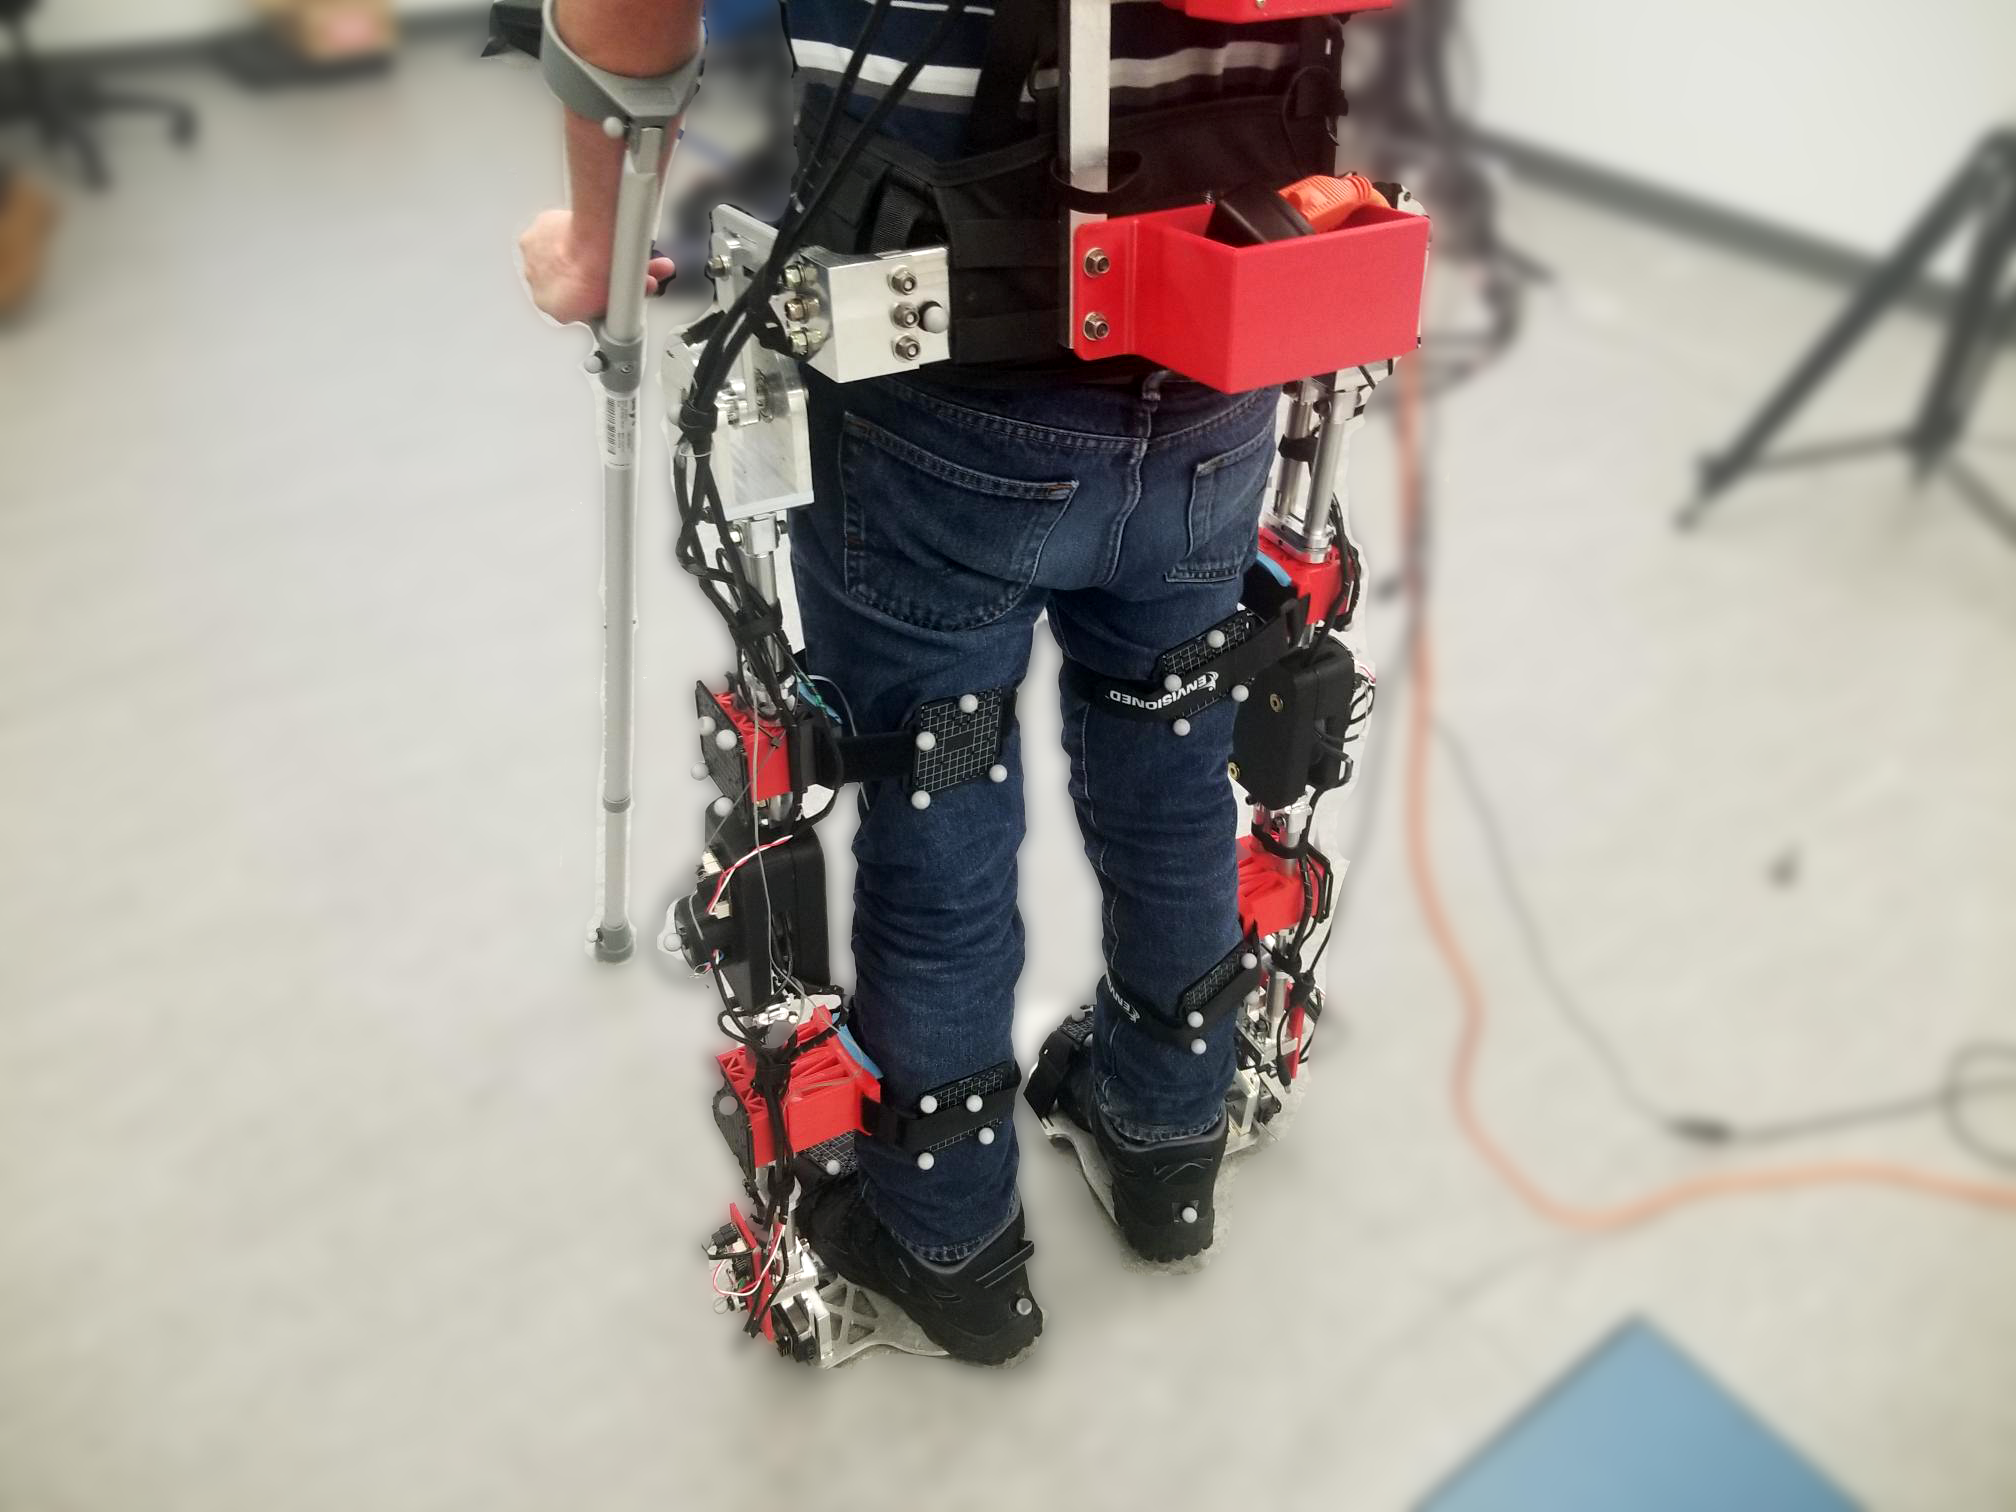
\includegraphics[scale=0.1, frame]{images/mech_design/exo_markers_back.png}}
        \caption[LARRE marker set back/side]{LARRE marker set back/side}
        \label{fig:larremarkerside}
    \end{subfigure}
    \begin{subfigure}{0.5\textwidth}
        \centering
        \captionsetup{justification=centering}
        \centerline{
        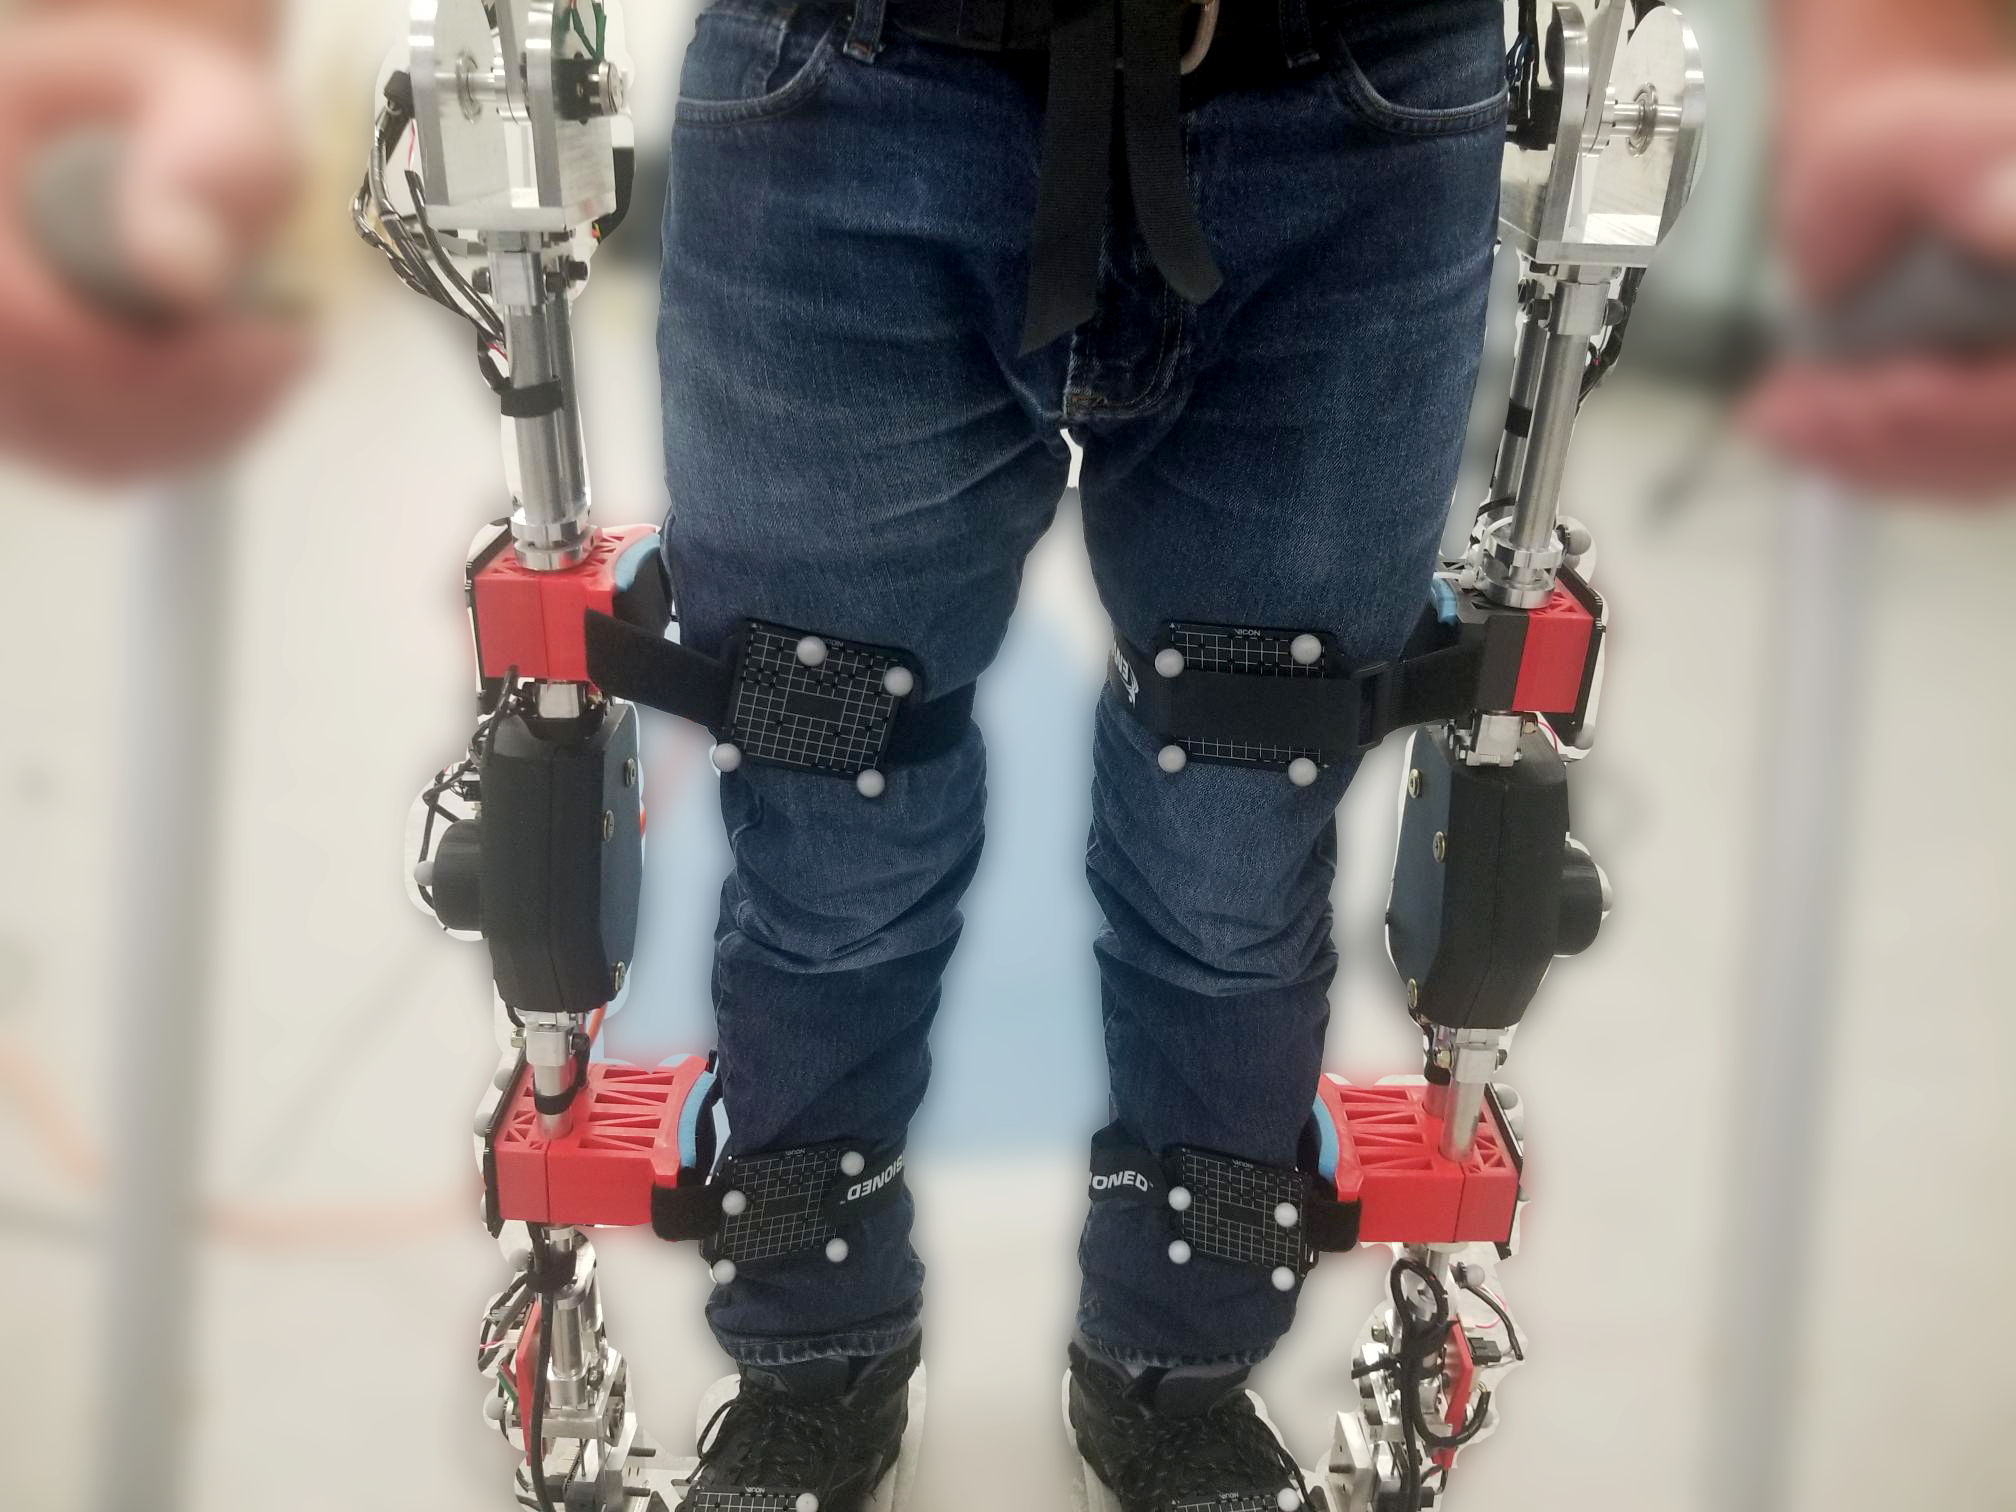
\includegraphics[scale=0.1, frame]{images/mech_design/exo_markers_front.png}}
        \caption[LARRE marker set front]{LARRE marker set front}
        \label{fig:larremarkerfront}
    \end{subfigure}    
    \caption{Marker set for LARRE}
    \label{fig:larremarker}
\end{figure}



\begin{figure}
    \begin{subfigure}{\textwidth}
        \centering
        \captionsetup{justification=centering}
        \centerline{
        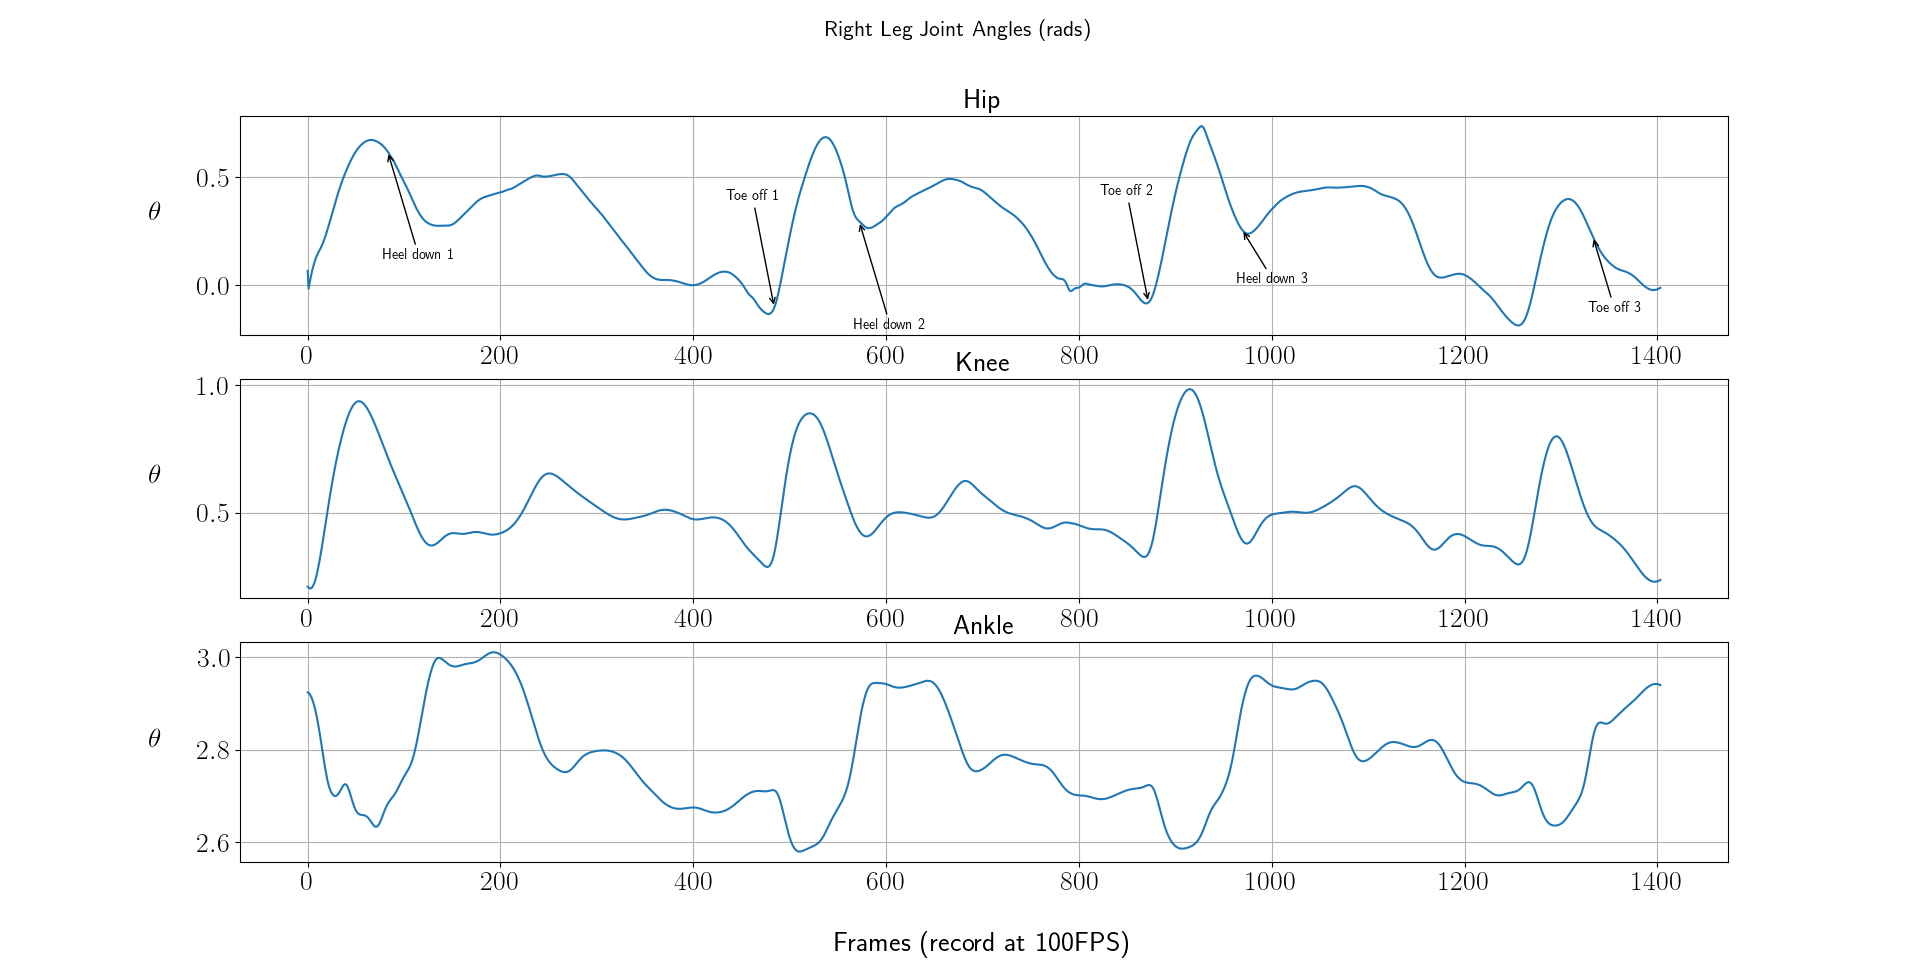
\includegraphics[width=\textwidth, frame]{images/mech_design/exo_joint_angles.png}}
        \caption[LARRE gait cycle angles]{Gait cycle angles of the LARRE}
        \label{fig:larregaitangles}
    \end{subfigure}
    \begin{subfigure}{\textwidth}
        \centering
        \captionsetup{justification=centering}
        \centerline{
        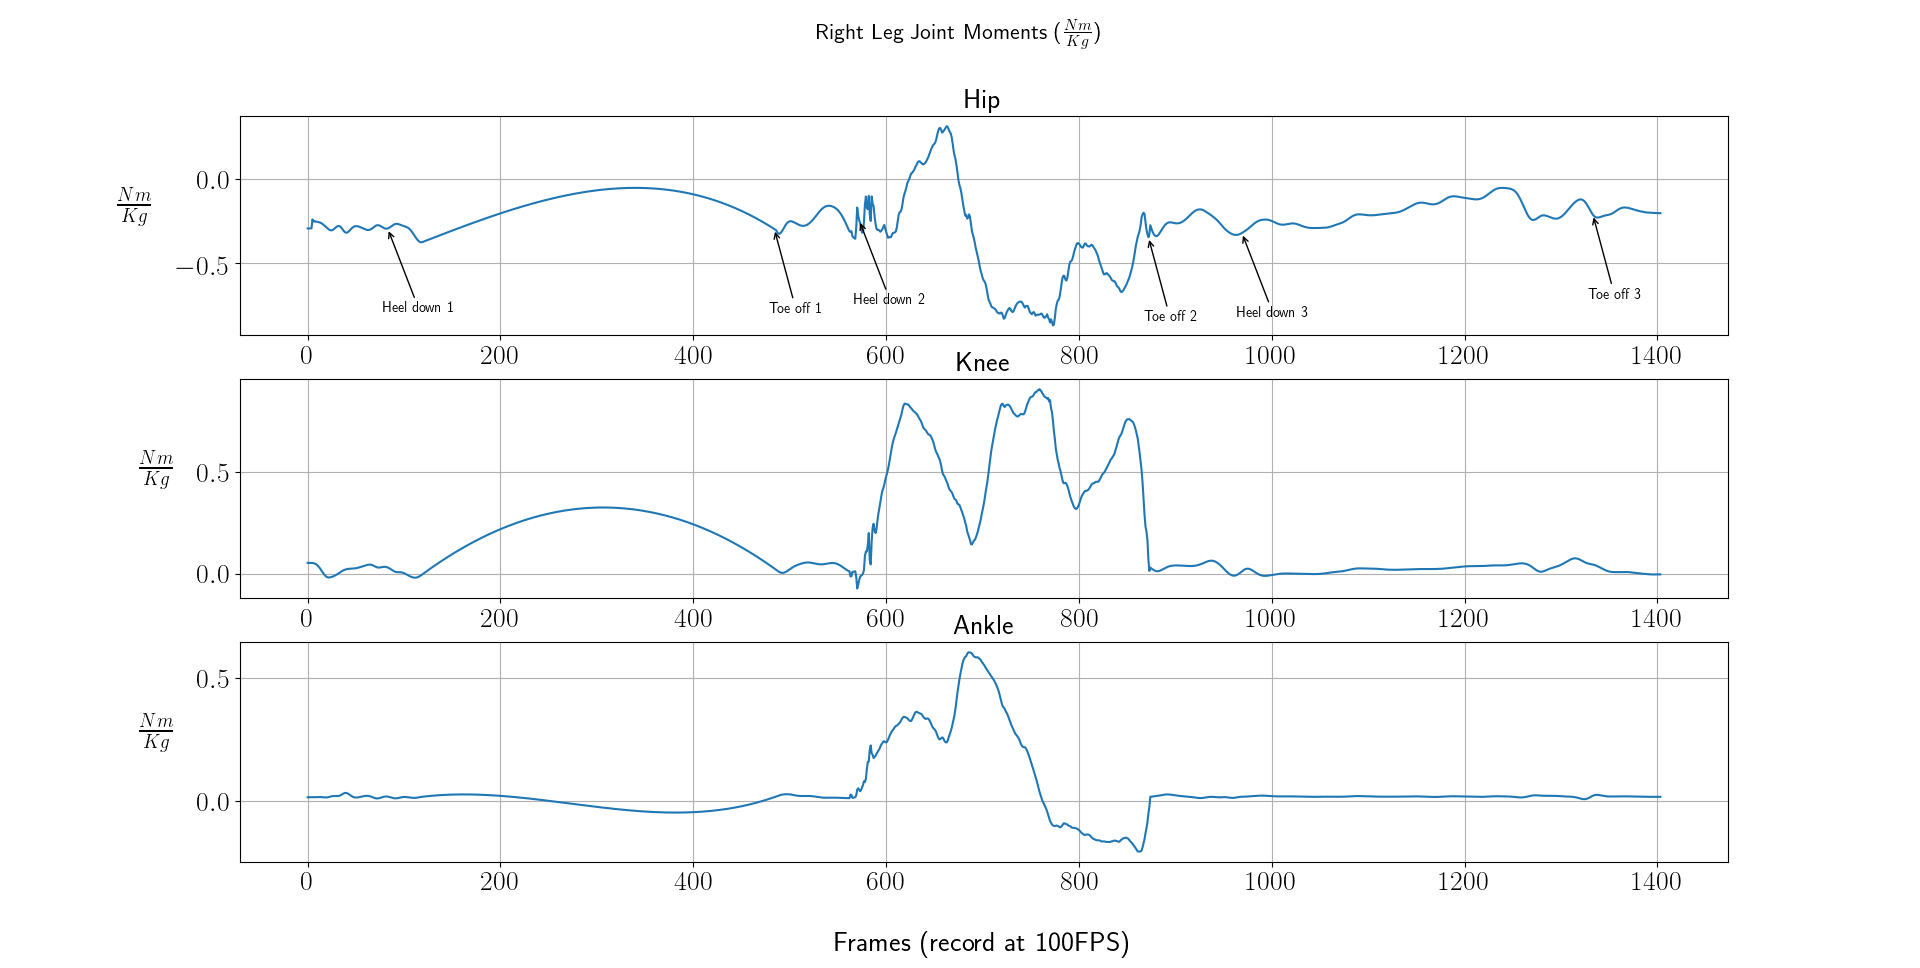
\includegraphics[width=\textwidth, frame]{images/mech_design/exo_joint_moments.png}}
        \caption[LARRE gait cycle moments]{Gait cycle moments of the LARRE}
        \label{fig:larregaitmoments}
    \end{subfigure}    
    \caption{Gait cycles kinematics for LARRE}
    \label{fig:exojointkin}
\end{figure}






% \begin{table}[h!]
% \begin{centering}
%     \begin{tabular}{ |p{1cm} p{2cm} p{2cm} p{2cm}|  }
%         \hline 
%         \multicolumn{4}{|c|}{LARRE Joints Limits} \\
%         \hline 
%         Joint & Flexion & Extension & Torque \\
%         \hline \hline
%         Hip   & $-60^{\circ}$   & $30^{\circ}$ &  60N \\
%         Knee &   $-110^{\circ}$  & $0$  & 50N \\
%         Ankle & $-20^{\circ}$ & $20^{\circ}$ &  - \\
%         \hline
%     \end{tabular}
%     \caption[LARRE Joint Limits]{Joint limits}    \centering
%     \label{tab:biomech}
% \end{centering}
% \end{table}